% Compilar com: latexmk -lualatex fatia2a.tex
\documentclass[11pt,a4paper]{article}
\usepackage[margin=2cm]{geometry}
\usepackage{fontspec}
\usepackage{unicode-math}
\setmainfont{Latin Modern Roman}
\setmathfont{Latin Modern Math}
\usepackage[brazil]{babel}
\usepackage{booktabs,tabularx,array,graphicx}
\usepackage{enumitem}
\usepackage{xurl}
\usepackage[colorlinks=true,linkcolor=blue!50!black,urlcolor=blue!50!black]{hyperref}
\setlength{\parindent}{0pt}
\setlength{\parskip}{0.5em}
\newcommand{\arq}[1]{\texttt{\nolinkurl{#1}}}

\title{Fatia 2a --- normalização de $dN/d\eta$ em $\eta\approx0$\\\large comparações entre detectores do RHIC}
\date{17 de novembro de 2026}
\author{}

\begin{document}
\maketitle
\vspace{-2em}

\section*{Dados e método}
\begin{itemize}[nosep]
\item Dados: \arq{../data/midrapidity_dndeta.csv} (260 linhas; PHOBOS, PHENIX, sPHENIX, BRAHMS; procedência em \arq{../data/README_data.md}).
\item Comparação de classes de centralidade \emph{idênticas}, mesmo sistema e energia: $r=\ln y_A-\ln y_B$.
\item PHOBOS: sistemáticos em 90\% C.L.\ divididos por $1{,}645$; janela $|\eta|<1$ convertida para $|\eta|<0{,}3$ com a forma
medida pelo sPHENIX (fator $1{,}020\pm0{,}004$, de $1{,}015$ em 0--3\% a $1{,}027$ em 60--65\%).
\item Por conjunto (par $\times$ sistema $\times$ energia): offset ponderado, inclinação linear em centralidade e
dispersão residual. Fração não correlacionada $f=\mathrm{rms}_{\mathrm{res}}/\sigma_{\mathrm{citado}}$ e $\rho_{\mathrm{ef}}=1-f^2$.
\item Script: \arq{fatia2a_normalizacao.py}; resultados: \arq{results.json}.
\end{itemize}

\begin{figure}[h]
\centering
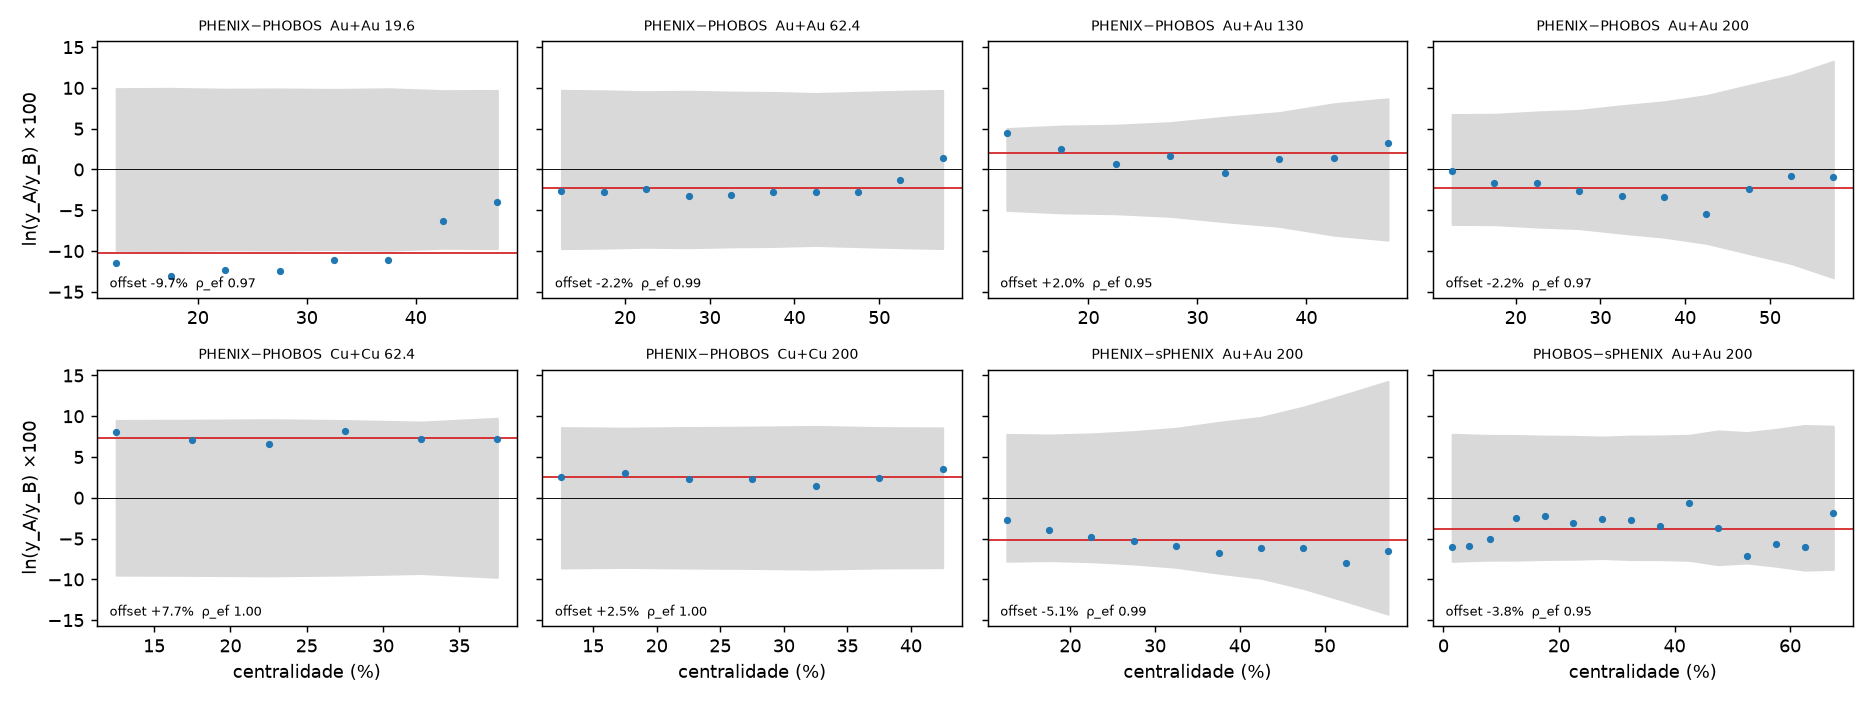
\includegraphics[width=\linewidth]{razoes_por_conjunto.png}
\caption{$\ln(y_A/y_B)$ por classe de centralidade. Faixa cinza: $\pm$ incerteza citada (soma em quadratura dos dois detectores).
Linha vermelha: offset ponderado. Os pontos formam curvas suaves, muito mais estreitas que a faixa: as incertezas citadas
são quase totalmente correlacionadas entre classes de centralidade.}
\end{figure}

\section*{Resultados}
\begin{tabularx}{\linewidth}{@{}l l r r r r r r r@{}}
\toprule
par & sistema & $\sqrt{s_{NN}}$ & $n$ & offset & $\sigma_{\mathrm{cit}}$ & pull & resíduo & $\rho_{\mathrm{ef}}$ \\
\midrule
BRAHMS--PHENIX & Au+Au & 130 & 2 & $-8{,}3\%$ & $7{,}9\%$ & $-1{,}09$ & --- & --- \\
BRAHMS--PHENIX & Au+Au & 200 & 2 & $-9{,}9\%$ & $10{,}2\%$ & $-1{,}02$ & --- & --- \\
PHENIX--PHOBOS & Au+Au & 19,6 & 8 & $-9{,}7\%$ & $9{,}8\%$ & $-1{,}03$ & $1{,}8\%$ & 0,97 \\
PHENIX--PHOBOS & Au+Au & 62,4 & 10 & $-2{,}2\%$ & $9{,}6\%$ & $-0{,}23$ & $1{,}0\%$ & 0,99 \\
PHENIX--PHOBOS & Au+Au & 130 & 8 & $+2{,}0\%$ & $6{,}5\%$ & $+0{,}31$ & $1{,}4\%$ & 0,95 \\
PHENIX--PHOBOS & Au+Au & 200 & 10 & $-2{,}2\%$ & $8{,}8\%$ & $-0{,}25$ & $1{,}5\%$ & 0,97 \\
PHENIX--PHOBOS & Cu+Cu & 62,4 & 6 & $+7{,}7\%$ & $9{,}5\%$ & $+0{,}78$ & $0{,}6\%$ & 1,00 \\
PHENIX--PHOBOS & Cu+Cu & 200 & 7 & $+2{,}5\%$ & $8{,}6\%$ & $+0{,}29$ & $0{,}6\%$ & 1,00 \\
PHENIX--sPHENIX & Au+Au & 200 & 10 & $-5{,}1\%$ & $9{,}7\%$ & $-0{,}54$ & $0{,}7\%$ & 0,99 \\
PHOBOS--sPHENIX & Au+Au & 200 & 15 & $-3{,}8\%$ & $7{,}9\%$ & $-0{,}49$ & $1{,}8\%$ & 0,95 \\
\bottomrule
\end{tabularx}

\textbf{Three-cornered hat, Au+Au 200} (PHENIX, PHOBOS, sPHENIX; 10 classes de 10--15\% a 55--60\%), componente
classe-a-classe (após remover offset e inclinação):
\begin{center}
\begin{tabular}{lccc}
\toprule
& PHENIX & PHOBOS & sPHENIX \\
\midrule
desvio classe-a-classe & 0,7\% & 1,5\% & 0,4\% \\
incerteza citada ($1\sigma$) & 7,4\% & 4,7\% & 6,2\% \\
\bottomrule
\end{tabular}
\end{center}

\section*{Leitura}
\begin{enumerate}
\item \textbf{2º momento --- estrutura de correlação medida.} Dentro de uma medida, o erro é quase totalmente correlacionado
entre classes de centralidade: $\rho_{\mathrm{ef}}=0{,}95$--$1{,}00$. A covariância é aproximadamente de posto 2
--- um \emph{offset} comum (tipo CS com $\rho\approx1$) e uma \emph{inclinação} em centralidade (determinação de centralidade;
até $\sim$20\% por 100\% de centralidade em 19,6 GeV) --- mais uma parte diagonal de $\sim$0,5--2\%.
Isto dá suporte empírico à escolha CS com $\rho=1$ do degrau 1, acrescido de um modo de inclinação.
\item \textbf{Magnitude.} Os offsets entre detectores ficam dentro das incertezas citadas (pull rms $\approx0{,}7$):
as incertezas publicadas (PHOBOS já em $1\sigma$) são, se algo, conservadoras.
\item \textbf{3º momento.} Assimetria dos resíduos padronizados: $-0{,}08\pm0{,}24$ (74 resíduos, bootstrap); dos offsets:
$+0{,}13$ com apenas 8 conjuntos. Compatível com zero; e, por diferenças, só a assimetria \emph{relativa} é identificável.
Nesta fatia não há sinal de não-gaussianidade.
\item \textbf{Ponto a verificar na calibração.} No arquivo da calibração (\arq{HIC_experimental_data/Au-Au-200/PHOBOS/dNdeta_eta_cen_00_03_PHOB.dat})
a incerteza relativa perto de $\eta=0$ é 6--7,5\%, compatível com o valor em 90\% C.L.\ do PHOBOS (7,5\% em $|\eta|<1$) e não
com $1\sigma$ ($\sim$4,6\%). \textbf{Possível}: o JETSCAPE usou os sistemáticos do PHOBOS em 90\% C.L.\ como se fossem $1\sigma$,
inflando-os por $\sim1{,}6\times$. Precisa ser confirmado nas tabelas por $\eta$ do PHOBOS.
\end{enumerate}

\section*{Ressalvas}
\begin{itemize}[nosep]
\item Conjuntos não são independentes (PHOBOS e PHENIX aparecem em vários); $N$ efetivo do offset $\approx7$.
\item A correção de janela em $\eta$ usa a forma de Au+Au 200 para todas as energias (incerteza dobrada fora de 200 GeV).
\item PHENIX/sPHENIX/BRAHMS publicam só incerteza total; o nível de confiança não é declarado (suposto $1\sigma$).
\item O desvio classe-a-classe do PHOBOS inclui o arredondamento dos valores tabelados e o ruído da correção de janela.
\end{itemize}
\end{document}
